
%mainfile: Multimodal_learning.tex

\title{Multimodal Learning: Examples in Gesture and Audio-Visual
Speech Recognition\vspace{-0.5em}}
\author{Hsieh Yu-Guan}
\date{\today}
\maketitle

\section*{Abstract}

\section{Introduction}

\section{Related Work}

\section{Presentation of Basic Network Architectures}

\section{Datasets and Preprocessing}

\subsection{Creative Senz3D}

\begin{figure}[H]
  \centering
  \hfill
  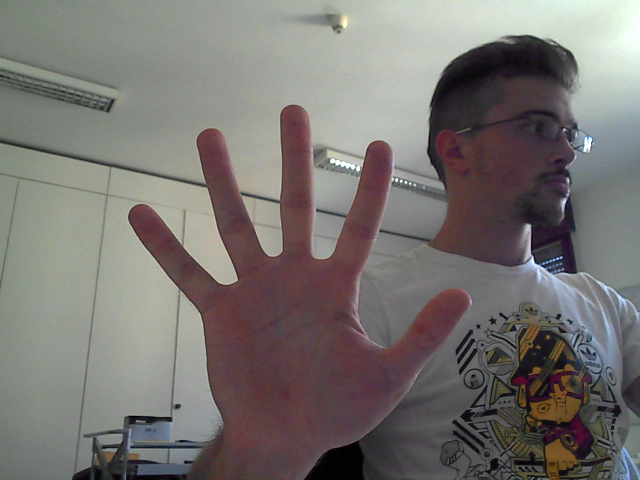
\includegraphics[width=0.23\linewidth]{dataset/senz3d/examples/1-color}
  \hfill
  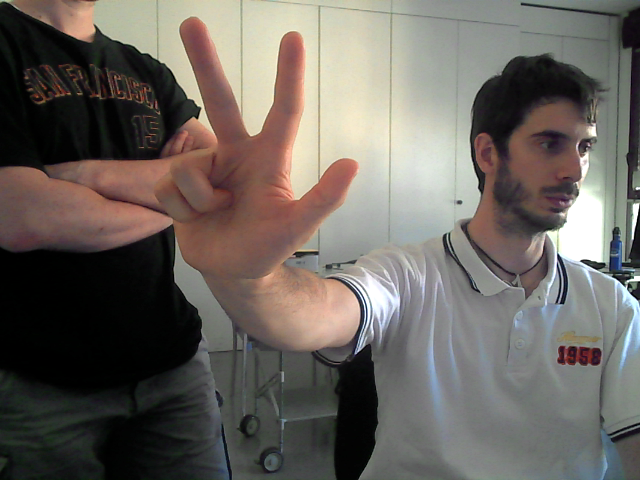
\includegraphics[width=0.23\linewidth]{dataset/senz3d/examples/12-color}
  \hfill
  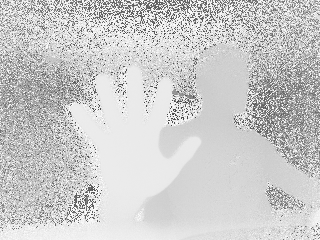
\includegraphics[width=0.23\linewidth]{dataset/senz3d/examples/1-depth}
  \hfill
  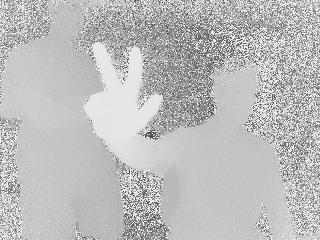
\includegraphics[width=0.23\linewidth]{dataset/senz3d/examples/12-depth}
  \caption{%
    \textbf{Example images in the Creative Senz3D dataset.}\\[0.1em]
    Left Two) Color images.\\[0.1em]
    Right Two) Corresponding depth images.\\[0.1em]
    All of the images are of size $480 \times 640$ and contain the
      the entire upper body of the subject.}
  \label{fig:senz3d_exs}
\end{figure}

\subsection{ASL Finger Spelling}

\begin{figure}[H]
  \centering
  \hfill
  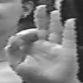
\includegraphics[width=0.15\linewidth]{%
    dataset/fingerspelling5/exs/or/g1}
  \hfill
  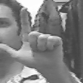
\includegraphics[width=0.15\linewidth]{%
    dataset/fingerspelling5/exs/or/g2}
  \hfill
  
\includegraphics[width=0.15\linewidth]{%
    dataset/fingerspelling5/exs/or/d3}
  \hfill
  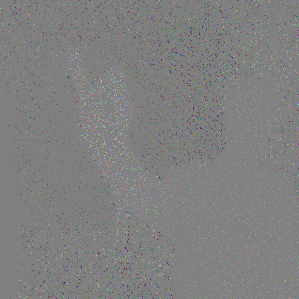
\includegraphics[width=0.15\linewidth]{%
    dataset/fingerspelling5/exs/or/d4}
  \hfill
  
\includegraphics[width=0.15\linewidth]{%
    dataset/fingerspelling5/exs/st/d1}
  \hfill
  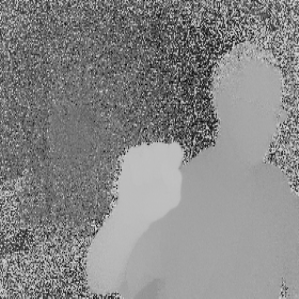
\includegraphics[width=0.15\linewidth]{%
    dataset/fingerspelling5/exs/st/d2}
  \caption{%
    \textbf{Example images in the ASL Finger Spelling dataset
      (after preprocessing).}\\[0.1em]
    Left Two) Grayscale intensity images.\\[0.1em]
    Middle Two) Depth maps after adjusting contrast.\\[0.1em]
    Right Two) Depth maps after Z-normalization.\\[0.1em]
    Images of this dataset have variable sizes, and they're all resized to
      $83 \times 83$ before being fed to the network. Generally only the
      hand region is contained in image.}
  \label{fig:fingerspelling_exs}
\end{figure}

\subsection{AVletters}

\begin{figure}[H]
  \centering
  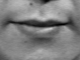
\includegraphics[width=0.15\linewidth]{%
    dataset/avletters/lips_no_data_aug/1}
  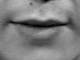
\includegraphics[width=0.15\linewidth]{%
    dataset/avletters/lips_no_data_aug/2}
  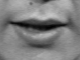
\includegraphics[width=0.15\linewidth]{%
    dataset/avletters/lips_no_data_aug/3}
  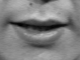
\includegraphics[width=0.15\linewidth]{%
    dataset/avletters/lips_no_data_aug/4}
  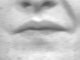
\includegraphics[width=0.15\linewidth]{%
    dataset/avletters/lips_no_data_aug/5}
  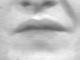
\includegraphics[width=0.15\linewidth]{%
    dataset/avletters/lips_no_data_aug/6}\\[0.15em]
  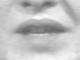
\includegraphics[width=0.15\linewidth]{%
    dataset/avletters/lips_no_data_aug/7}
  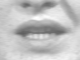
\includegraphics[width=0.15\linewidth]{%
    dataset/avletters/lips_no_data_aug/8}
  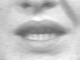
\includegraphics[width=0.15\linewidth]{%
    dataset/avletters/lips_no_data_aug/9}
  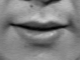
\includegraphics[width=0.15\linewidth]{%
    dataset/avletters/lips_no_data_aug/10}
  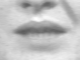
\includegraphics[width=0.15\linewidth]{%
    dataset/avletters/lips_no_data_aug/11}
  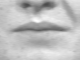
\includegraphics[width=0.15\linewidth]{%
    dataset/avletters/lips_no_data_aug/12}
  \caption{%
    \textbf{Example visual input for the AVletters dataset
      (left to right, top to bottom).}\\[0.1em]
    Pre-extracted lip regions of $60 \times 80$ pixels are provided.
      Each image sequence is resampled to be of length twelve in order to
      give an input of fixed size to the network.}
  \label{fig:avletters_exs}
\end{figure}

\section{Experimental Setup}

\section{Experiences and Results: Unimodal Cases}

\subsection{Classification}

\begin{figure}[H]
  \centering
  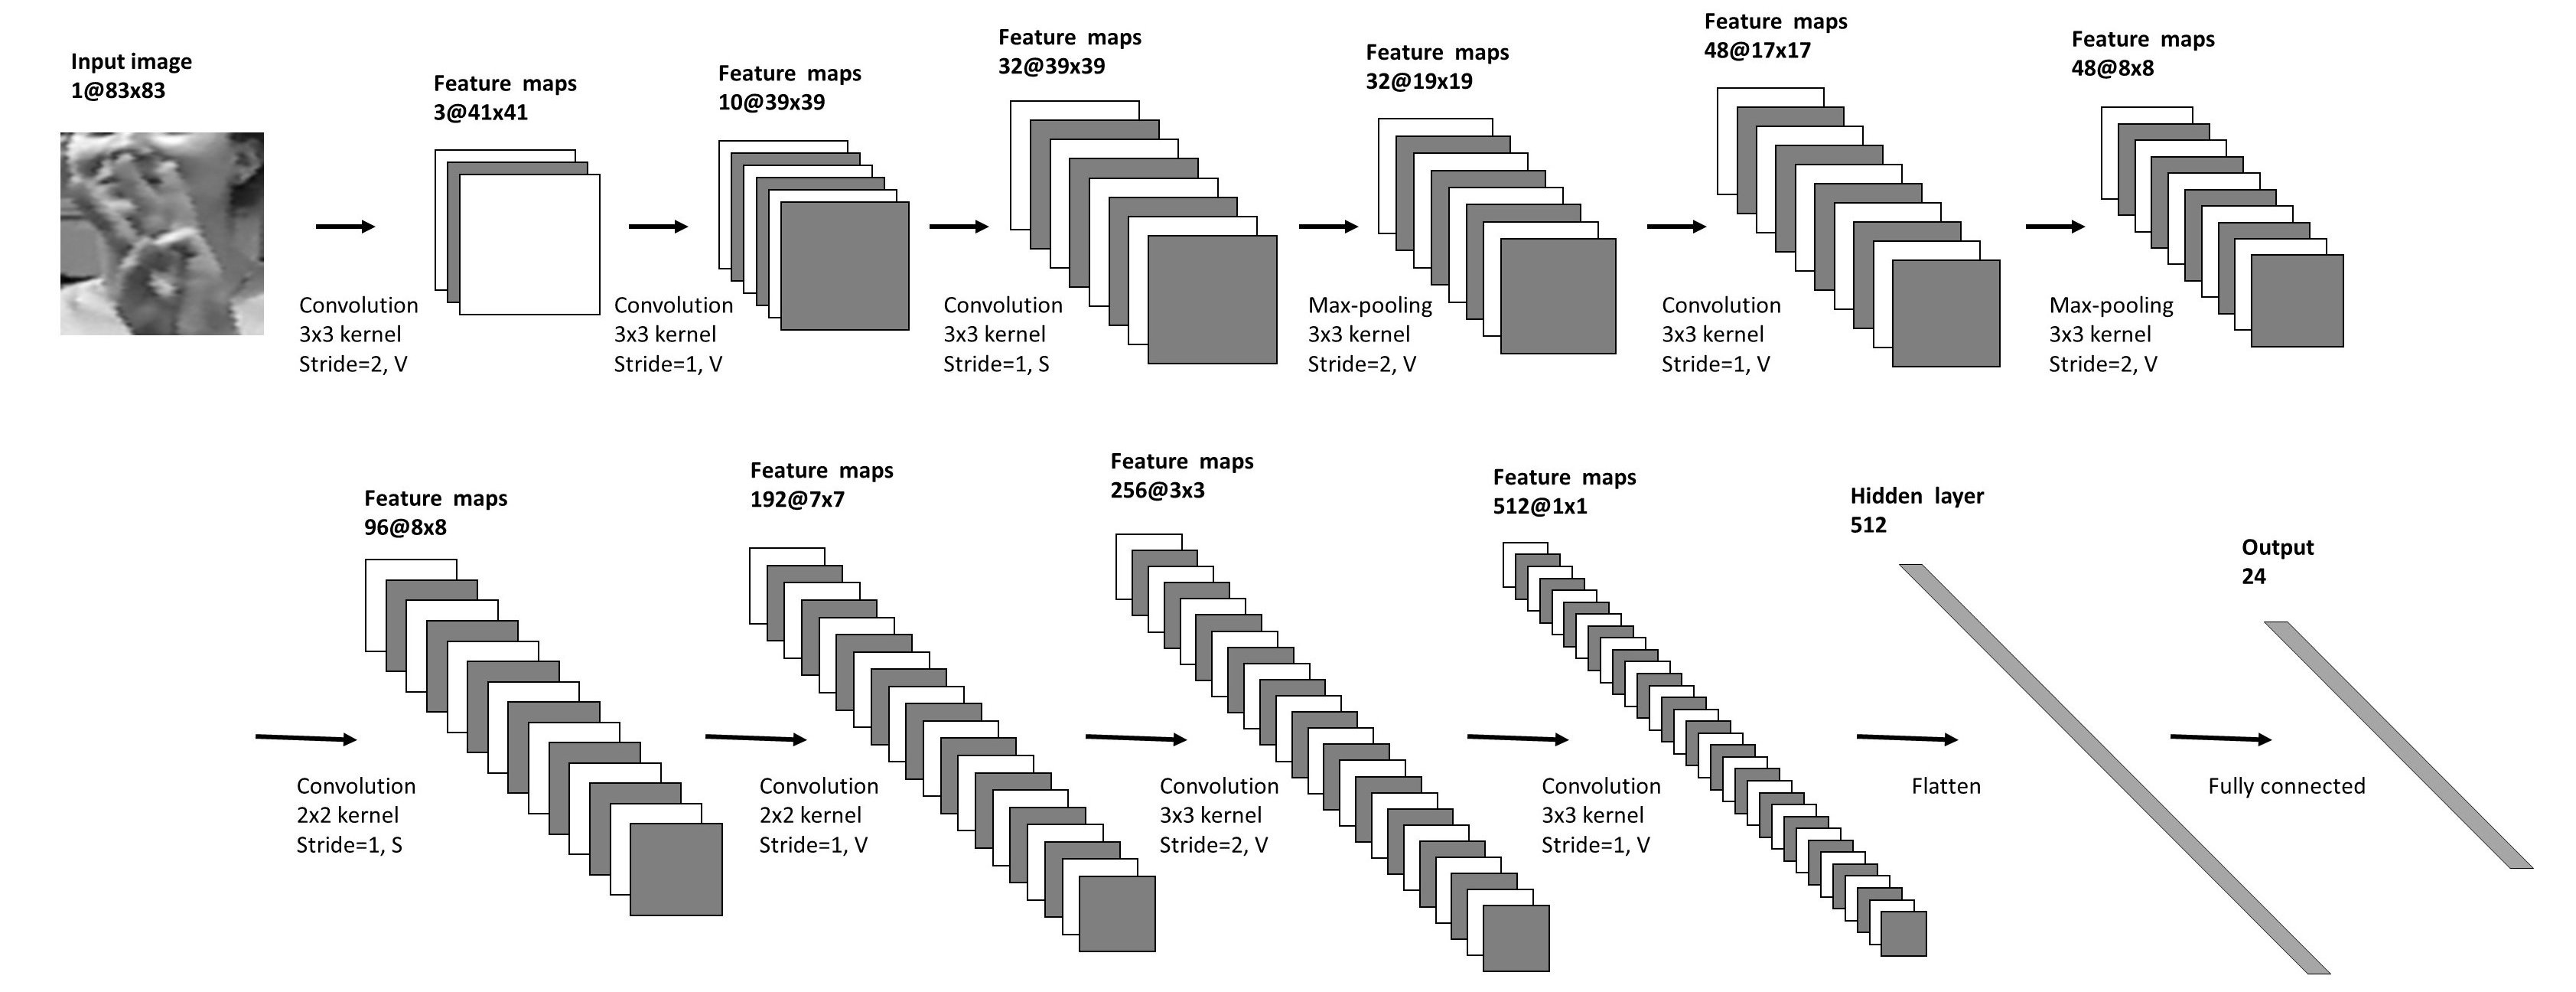
\includegraphics[width=\linewidth]{architectures/CNN10}\\[-1.5em]
  \caption{%
    \textbf{CNN architecture used for the Finger Spelling  dataset.}
      \\[0.1em]
    The input of the nework is a one-channel image of size $83 \times 83$.
      It contains ten hidden layers. S stands for `SAME' padding
      and V stands for `VALID' padding (see text).}
  \label{fig:CNN10}
\end{figure}

\subsection{Convolutional auto-encoder}

\begin{figure}[H]
  \centering
  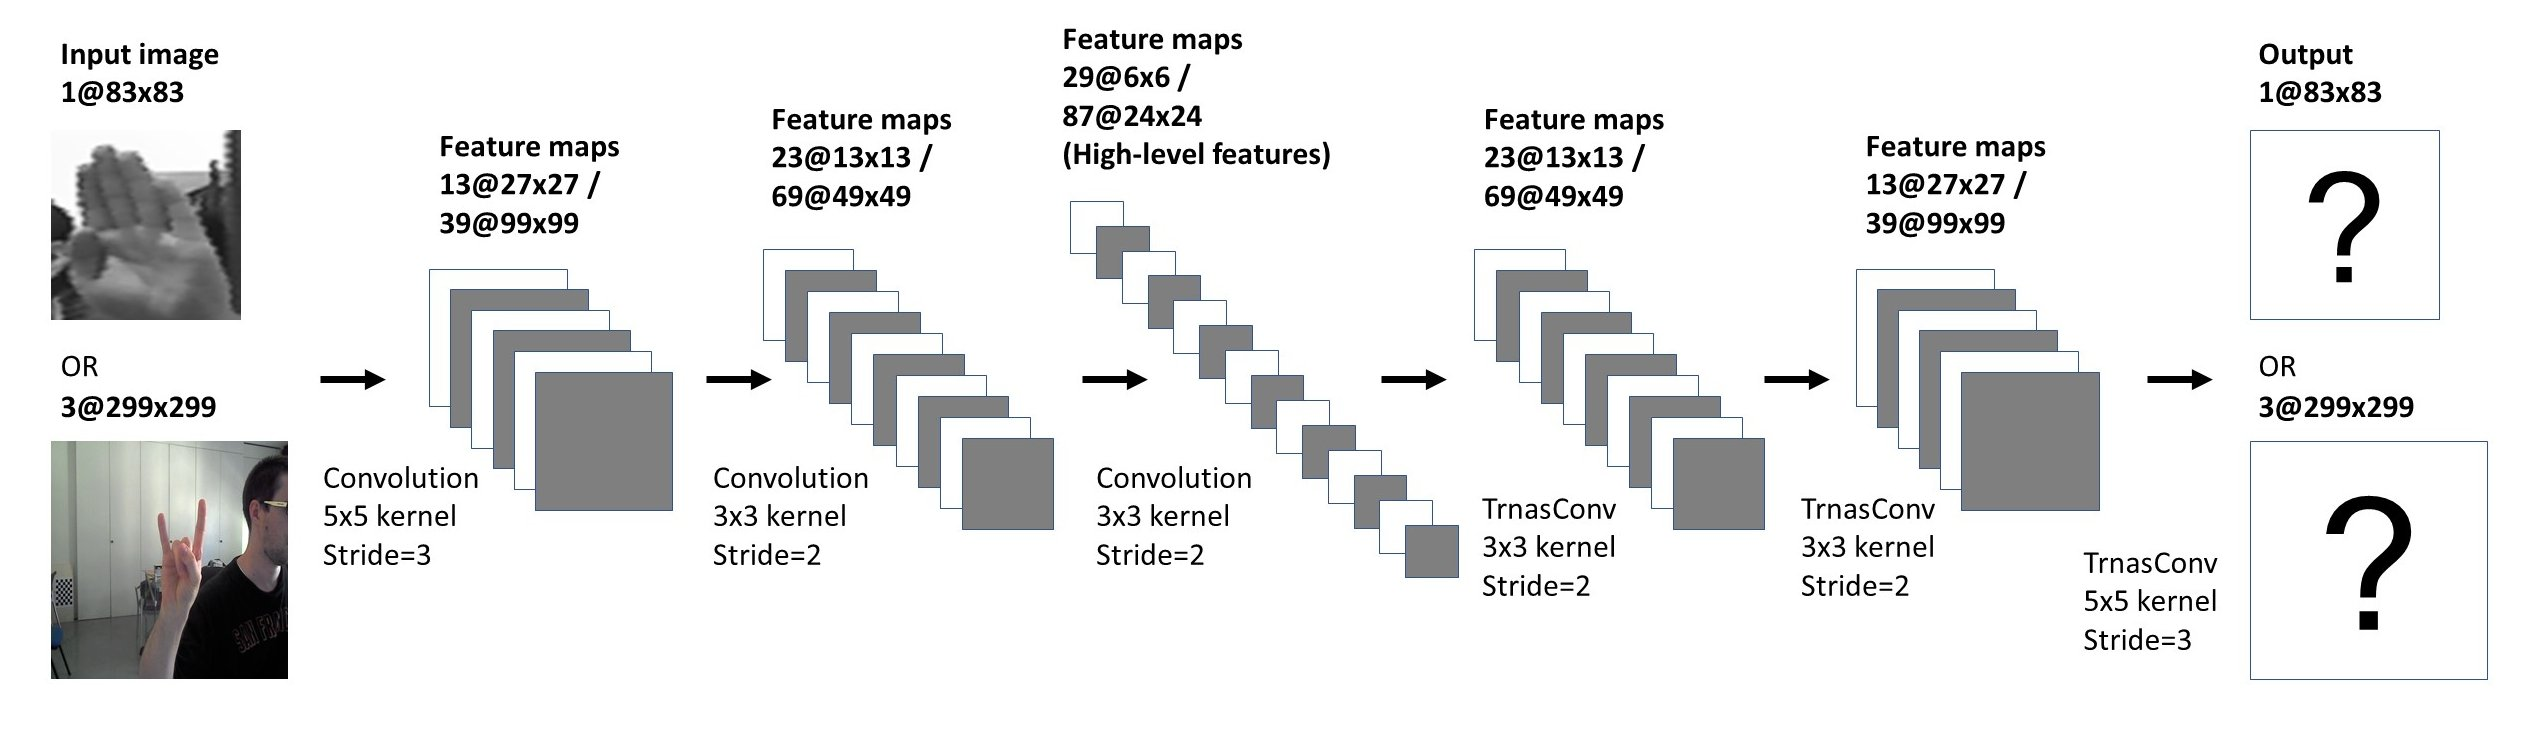
\includegraphics[width=\linewidth]{architectures/CAE5}\\[-2.5em]
  \caption{%
    \textbf{Convolutional auto-encoder architecture with 
      three convolutional layers and three tranposed convolutional
      layer.}\\[0.1em]
    Activation values of the middle layer are taken as 
      high-level features of the input image. Inputs of the network
      can be of different sizes. We only use valid paddings here.}
  \label{fig:CAE5}
\end{figure}

\begin{figure}[H]
  \centering
  \hfill
  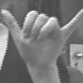
\includegraphics[width=0.28\linewidth]{%
    dataset/fingerspelling5/gray/gray4}
  \hfill
  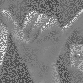
\includegraphics[width=0.28\linewidth]{%
    dataset/fingerspelling5/gray/gray_dropout4}
  \hfill
  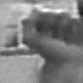
\includegraphics[width=0.28\linewidth]{%
    dataset/fingerspelling5/gray/gray_reconstruction4}
  \caption{%
    \textbf{Image restoration using convolutional auto-encoder.}\\[0.1em]
      Left) Clean Image.\\[0.1em]
      Middle) Noisy image [input].\\[0.1em]
      Right) Restored image [output].}
  \label{fig:image_restoration}
\end{figure}

\section{Experiences and Results: Multimodal Cases}

\subsection{Learning shared representation}

\begin{figure}[H]
  \centering
  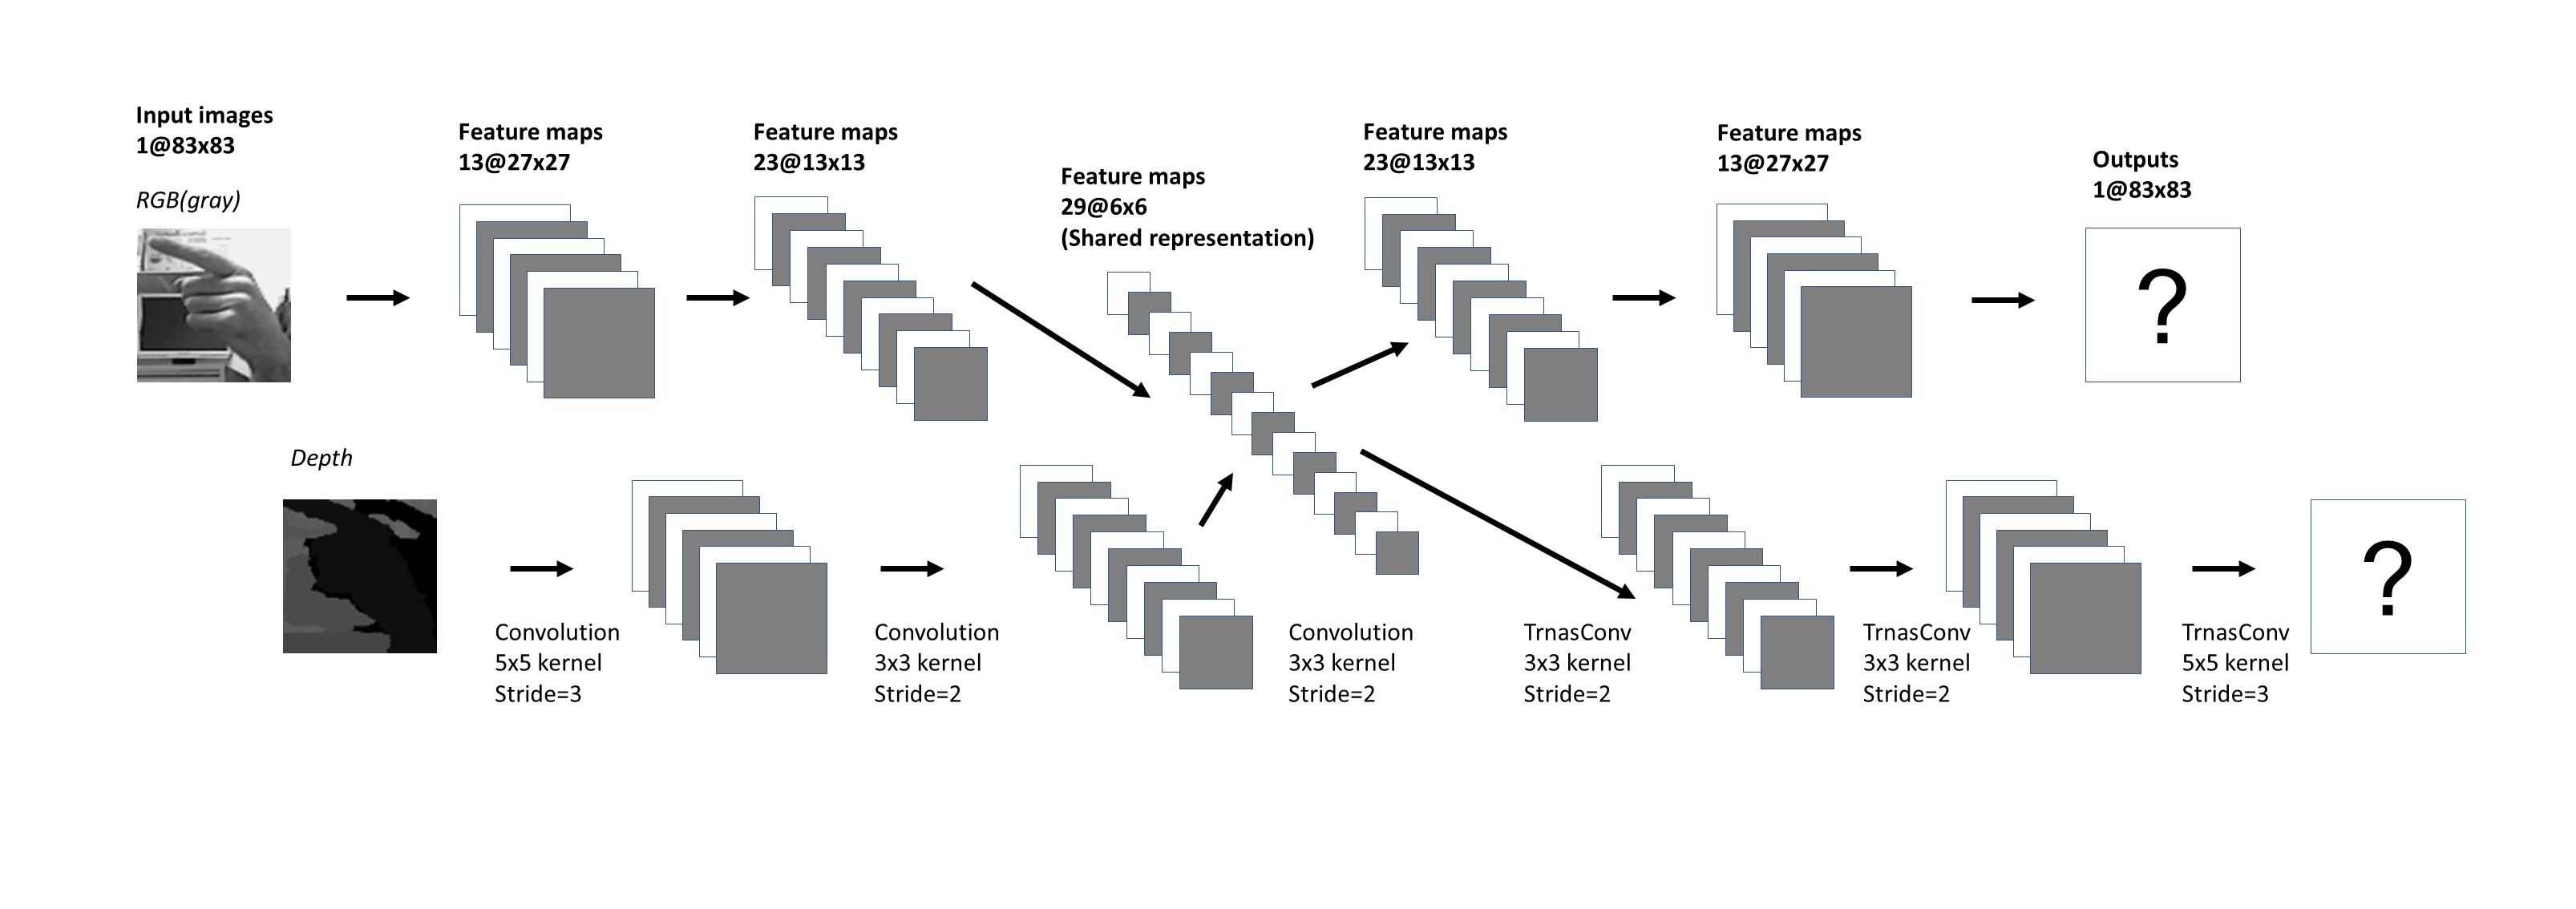
\includegraphics[width=\linewidth]{architectures/FAE5}\\[-2.5em]
  \caption{%
    \textbf{The bimodal convolutional auto-encoder model that is
      used to learn shared multimodal representation.}\\[0.1em]
    We simply take the CAE architecture that is introduced earlier
      (\autoref{fig:CAE5}) for each modaliy but force them to have a
      shared middle layer by adding the corresponding activation values.
      We then try to reconstruct the two images separately through
      two disjoint paths.}
  \label{fig:FAE5}
\end{figure}

\begin{figure}[H]
  \centering
  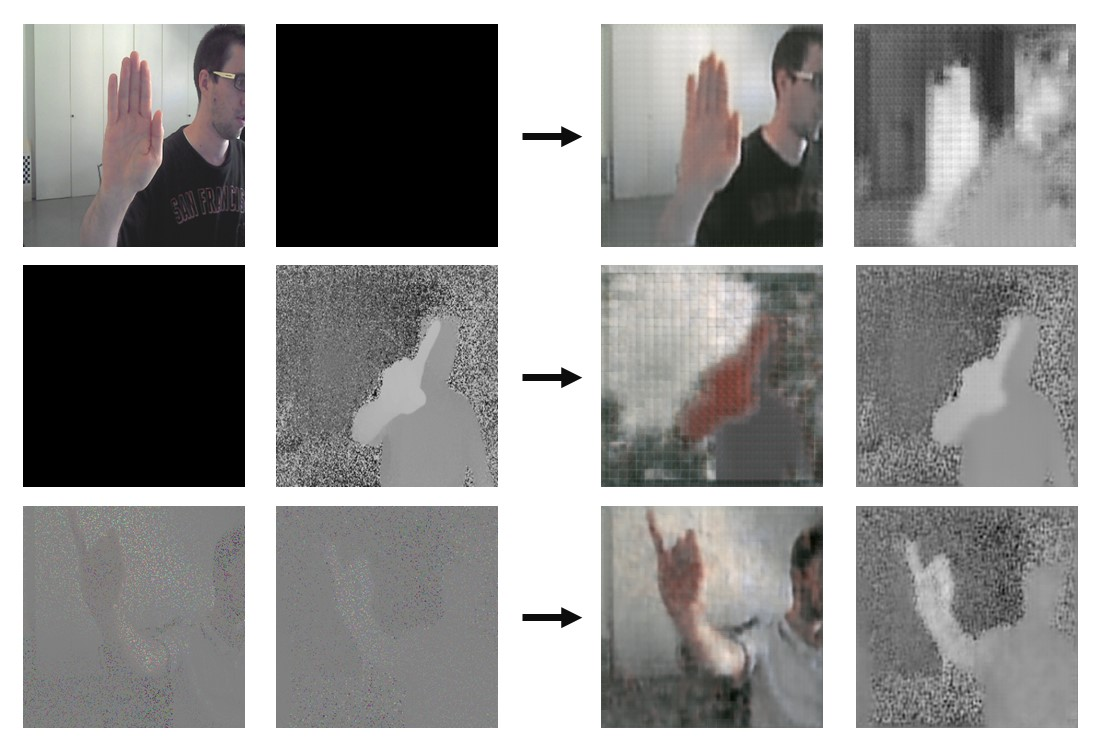
\includegraphics[width=\linewidth]{dataset/senz3d/reconstructions}\\[-1em]
  \caption{%
    \textbf{Restore color and depth images from incomplete input
      information.}\\[0.1em]
      Top) Only the color image is given.\\[0.1em]
      Middle) Only the depth image is given.\\[0.1em]
      Botttom) Both modalities are given but with little information
        (10\% of pixels).}
  \label{fig:color_depth_restoration}
\end{figure}

\subsection{Transfer learning}


\newpage

\begin{thebibliography}{99}

\bibitem{M. Asadi-Aghbolaghi 2017}
  17. M. Asadi-Aghbolaghi, A. Clapés, M. Bellantonio, H. J. Escalante, 
  V. Ponce-López, X. Baró, I. Guyon, S. Kasaei, and S. Escalera. 
  A Survey on Deep Learning Based Approaches for Action and Gesture 
  Recognition in Image Sequences. 
  In \textit{Automatic Face \& Gesture Recognition (FG 2017) 2017 12th IEEE
  International Conference}, 2017.

\bibitem{T. Baltrusaitis 2017}
  T. Baltrusaitis, C. Ahuja and L-P. Morency. Multimodal Machine Learning:
  A Survey and Taxonomy. In \textit{CoRR}, vol. abs/1705.09406, 2017.

\bibitem{C. Bregler 1994}
  C. Bregler and Y. Konig. "Eigenlips" for robust speech recognition.
  In \textit{ICASSP}, 1994.

\bibitem{L. Deng 2013}
  L. Deng, G. Hinto and B. Kinsbury. New types of deep neural network
  learning for speech recognition and related applications: An overview.
  In \textit{ICASSP}, 2013.

\bibitem{A. Droniou 2014}
  A. Droniou, S. Ivaldi, and O. Sigaud. A deep unsupervised network
  for multimodal perception, representation and classification. In
  \textit{Robotics and Autonomous System}, 2014.

\bibitem{A. Frome 2013}
  A. Frome, G. S. Corrado, J. Shlens, S. Bengio, J. Dean,
  T. Mikolov, et al. Devise: A deep visual-semantic embedding model. 
  In \textit{NIPS}, 2013.

\bibitem{G. Hinton 2012}
  G. Hinton, L. Deng, D. Yu, G. Dahl, A. Mohamed, N. Jaitly, A. Senior, V.
  Vanhoucke, P. Nguyen, T. Sainath and B. Kingsbury. Deep neural networks
  for acoustic modeling in speech recognition.
  In \textit{IEEE Signal Processing Mag} Vol. 29, 2012.

\bibitem{S. Ioffe 2015}
  S. Ioffe and C. Szegedy. Batch normalization, accelerating deep network
  training by reducing internal covaraiate shift. In \textit{CoRR},
  vol. abs/1502.03167, 2015.

\bibitem{A. K. Katsuaggelos 2015}
  A. K. Katsaggelos, S. Bahaadini and R. Molina. Audiovisual fusion:
  Challenges and new approaches. In \textit{Proceedings of the IEEE},
  vol. 103, 2015.

\bibitem{A. Krizhevsky 2012}
  A. Krizhevsky, I. Sutskever, and G. E. Hinton.  ImageNet Classification
  with Deep Convolutional Neural Networks. In \textit{NIPS}, 2012.

\bibitem{J. Masci 2011}
  J. Masci, U. Meier, D. C. ̧san, and J. Schmidhuber.
  Stacked convolutional auto-encoders for hierarchical feature extraction.
  In \textit{Artificial Neural Networks and Machine Learning–ICANN}, 2011.

\bibitem{I. Matthews 2002}
  I. Matthews, T. F. Cootes, J. A. Bangham and S. Cox. Extraction of visual
  features for lipreading. In \textit{PAMI}, 2002.

\bibitem{A. Memo 2015}
  A. Memo, L. Minto and P. Zanuttigh.  Exploiting Silhouette Descriptors and
  Synthetic Data for Hand Gesture Recognition. In \textit{STAG: Smart
    Tools \& Apps for Graphics}, 2015.

\bibitem{A. Memo 2017}
  A. Memo and P. Zanuttigh. Head-mounted gesture controlled interface
  for human-computer interaction. In \textit{Multimedia Tools and
  Applications}, 2017.

\bibitem{S. Mitra 2007}
  S. Mitra and T. Acharya. Gesture recognition: A survey. 
  In \textit{IEEE Systems, Man, and Cybernetics}, 37:311–324, 2007. 

\bibitem{P. Molchanov 2015}
  P. Molchanov, S. Gupta, K. Kim, and J. Kautz. Hand gesture recognition 
  with 3D convolutional neural networks. In \textit{CVPRW}, 2015.

\bibitem{S. Moon 2015}
  S. Moon, S. Kim and H. Wang. Multimodal transfer deep learning with
    applications in audio-visual recognition. In \textit{NIPS MMML
    Workshop}, 2015.

\bibitem{J. Nagi 2011}
  J. Nagi, F. Ducatelle, G. Di Caro, D. Ciresan, U. Meier, A. Giusti,
  F. Nagi, J. Schmidhuber, and L. Gambardella.
  Max-pooling convolutional neural networks for vision-based hand 
  gesture recognition.
  In \textit{Proceedings of the IEEE International Conference on
  Signal and Image Processing Applications}, 2011.

\bibitem{N. Neverova 2014}
  N. Neverova, C. Wolf, G. W. Taylor, and F. Nebout.  Multiscale deep
  learning for gesture detection and localization. In \textit{ECCVW}, 2014.

\bibitem{J. Ngiam 2011}
  J. Ngiam, A. Khosla, M. Kim, J. Nam, and A. Y. Ng. 
  Multimodal deep learning. In:
  In \textit{International Conference on Machine Learning}.  28. 
  Bellevue, Washington, USA, 2011.

\bibitem{K. Noda 2014}
  K. Noda, Y. Yamaguchi, K. Nakadai, H. G. Okuno and T. Ogata. Audio-visual
  speech recognition using deep learning.  In \textit{Applied Intelligence,
  vol. 42, no. 4, pp. 722–737, 2014.}

\bibitem{E. Petahan 1988}
  E. Petahan, B. Bischoff, D. Bodoff, and N. M. Brooke. An Improved
  Automatic Lipreading System to enhance Speech Recognition.
  In \textit{ACM SIGCHI}, 1988.

\bibitem{L. Pigou 2014}
 L. Pigou, S. Dieleman, P. J. Kindermans, and B. Schrauwen.
  Sign language recognition using convolutional neural networks. In
  \textit{Workshop at the European Conference on Computer Vision},
  pages 572--578, 2014.

\bibitem{G. Potamianos 2004}
  G. Potamianos, C. Neti, J. Luettin and  I. Matthews. Audio-visual
  automatic speech recognition: An overview. In \textit{Issues in Visual
  and Audio-Visual Speech Processing, MIT Press}, 2004.

\bibitem{N. Pugeault 2011}
  N. Pugeault, and R. Bowden. Spelling It Out: Real-Time ASL
  Fingerspelling Recognition. In \textit{Proceedings of the 1st IEEE
  Workshop on Consumer Depth Cameras for Computer Vision}, 2011.

\bibitem{R. Socher 2013}
  R. Socher, M. Ganjoo, H. Sridhar, O.Bastani, C. D. Manning, and
  A. Y. Ng. Zero-shot learning through cross-modal transfer.
  In \textit{International Conference on Learning Representations (ICLR)},
  Scottsdale, Arizona, USA, 2013.

\bibitem{N. Srivastava 2014}
  N. Srivastava, G. Hinton, A. Krizhevsky, I. Sutskever and R. Salakhutdinov.
  Dropout: A simple way to prevent neural networks from overfitting. In
  \textit{Journal of Machine Learning Research}, vol. 15, 2014.

\bibitem{T. Starner 1998}
  T. Starner, A. Pentland, and J. Weaver. Real-time american sign language
  recognition using desk and wearable computer based video. 
  In \textit{PAMI}, 20(12):1371–1375, 1998.

\bibitem{J. Sung 2015}
  J. Sung, I. Lenz, and A. Saxena. Deep multimodal embedding:
  Manipulating novel objects with point-clouds, language and trajectories.
  In \textit{CoRR}, vol. abs/1509.07831, 2015.

\bibitem{C. Szegedy 2016}
  C. Szegedy, S. Ioffe, V, Vanhoucke. Inception-v4, inception-ResNet and the
  impact of residual connections on learning. In \textit{CoRR},
  vol. abs/1602.07261, 2016.

\bibitem{V. Turchenko 2017}
  V. Turchenko, E. Chalmers and A. Luczak. A deep convolutional auto-encoder
  with pooling - unpooling layers in Caffe. In \textit{CoRR},
  vol. abs/1701.04949, 2017.

\bibitem{J. Weston 2010}
  J. Weston, S. Bengio, and N. Usunier. 
  Large scale image annotation: learning to rank with joint word-image
  embeddings. In \textit{Machine Learning}, 81(1):21--35, 2010.

\bibitem{Di Wu 2016}
  Di Wu, Lionel Pigou, Pieter-Jan Kindermans, Nam Do-Hoang Le, Ling Shao,
  Joni Dambre, and Jean-Marc Odobez. 
  Deep Dynamic Neural Networks for Multimodal Gesture Segmentation and
  Recognition. In \textit{Pattern Analysis and Machine Intelligence
  IEEE Transactions}, vol. 38, 2016.

\bibitem{B. P. Yuhas 1989}
  B. P. Yuhas, M. H. Goldstein, and T. J. Sejnowski. Integration of acoustic
  and visual speech signals using neuralnetworks. in \textit{IEEE Comm.
  Magazine}, pp. 65--71, 1989.

\end{thebibliography}
